\section{Curve in $\mathbb{R}^3$}

\begin{definition}[Curva]
    Una \textbf{curva} in $\mathbb{R}^3$ è definita come un'appliciazione continua da un intervallo aperto $U \subset \mathbb{R}$ nella sua immagine $\mathbb{R}^3$
    ovvero, utilizzando le notazioni introdotte nella Sezione \ref{sec:1_vettori}:
\end{definition}

\begin{minipage}
    {0.45\textwidth}
    \begin{equation*}
        \vec r(t): U \subset \mathbb{R} \to \mathbb{R}^3
    \end{equation*}
    \\[1em]
    \begin{equation*}
        \vec r (t) =  \begin{pmatrix}
        x(t)\\
        y(t)\\
        z(t)
        \end{pmatrix}= x(t)\hat i + y(t)\hat j + z(t)\hat k
    \end{equation*}
\end{minipage}
\begin{minipage}
    {0.45\textwidth}
    \begin{figure}[H]
    \centering
    \begin{tikzpicture}[scale=1]

    %-------------------------
    % Assi cartesiani
    %-------------------------
    \draw[->, thick] (0,0) -- (4,0) node[right] {$y$};
    \draw[->, thick] (0,0) -- (0,4) node[above] {$z$};
    \draw[->, thick] (0,0) -- (-2,-2) node[below] {$x$};

    % Versori in rosso
    \draw[->, very thick, red] (0,0) -- (0,1.2);
    \node[left, red] at (0,0.9) {$\hat{k}$};

    \draw[->, very thick, red] (0,0) -- (1.2,0);
    \node[below, red] at (0.9,0) {$\hat{j}$};

    \draw[->, very thick, red] (0,0) -- (-0.9,-0.9);
    \node[below left, red] at (-0.6,-0.6) {$\hat{i}$};

    %-------------------------
    % Curva r(t)
    %-------------------------
    \draw[blue, thick, domain=-1:3.5, smooth]
    plot (\x, {2 + 0.8*sin(1.2*\x r) - 0.5*cos(2*\x r)});

    \node[blue] at (3.5,2.6) {$\vec r(t)$};

    % Punto sulla curva
    \filldraw[blue] (2.3,2.2) circle (3pt);

    % Proiezione tratteggiata
    \draw[blue, dashed, thick] (2.3,2.2) -- (2.3,-1.5);

    %-------------------------
    % Asse del parametro t
    %-------------------------
    \draw[->, thick] (0.5,-1.5) -- (4.5,-1.5) node[right] {$t$};

    % Tacche a e b
    \draw (1.2,-1.3) -- (1.2,-1.7);
    \node[below] at (1.2,-1.7) {$a$};

    \draw (3.2,-1.3) -- (3.2,-1.7);
    \node[below] at (3.2,-1.7) {$b$};

    % Punto nell'intervallo
    \filldraw[blue] (2.3,-1.5) circle (3pt);

    % Parentesi graffa intervallo
    \draw[blue]
    (1.2,-2.1) -- (1.2,-2.3)
    -- (2.2,-2.5)
    -- (3.2,-2.3)
    -- (3.2,-2.1);

    \node[blue] at (2.2,-2.8) {$U$};

    \end{tikzpicture}
    \end{figure}
\end{minipage}

La coppia $(t, U)$ dove $t$ è la variabile $t\in U$ utilizzata per percorrere la curva, è detta \textbf{parametrizzazione} della curva. 
La variabile $t$ è detta \textbf{ascissa curvilinea} o parametro d'arco, mentre $U$ è detto \textbf{dominio} della curva. L'insieme $\vec r(U) \subset \mathbb{R}^3$ è detto \textbf{immagine} della curva.

\begin{example}[Parabola]
    La parabola è una curva che può essere rappresentata da una parametrizzazione del tipo:
    \begin{equation*}
        \vec r(t) = t\hat i + t^2 \hat j + 0\hat k
    \end{equation*}
    con $t \in \mathbb{R}$. In questo caso, il dominio $U$ è l'intero insieme dei numeri reali, e l'immagine della curva è l'insieme dei punti $(t, t^2, 0)$ che formano una parabola nel piano $xy$.

    \begin{figure}[H]
    \centering
    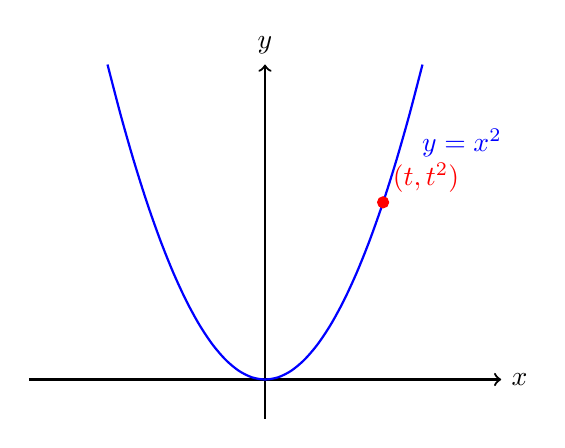
\begin{tikzpicture}[scale=1]
    
    % Assi
    \draw[->, thick] (-3,0) -- (3,0) node[right] {$x$};
    \draw[->, thick] (0,-0.5) -- (0,4) node[above] {$y$};
    
    % Parabola
    \draw[blue, thick, domain=-2:2, smooth] plot (\x, {\x*\x});
    \node[blue] at (2.5,3) {$y = x^2$};
    
    % Punto di esempio
    \filldraw[red] (1.5,2.25) circle (2pt);
    \node[red, above right] at (1.5,2.25) {$(t, t^2)$};
    
    \end{tikzpicture}
    \end{figure}
    
\end{example}